% !TEX root = ../thesis-example.tex
%
\section{Hyperledger-based Application}
\label{sec:impr:hl}



With the interfaces needed to easily expand the system being in place, we deemed it a good next step to add another Blockchain protocol. Specifically, we chose \emph{Hyperledger}. The application was successfully expanded with all necessary components built and tested, although the front-end still has problems trying to pack this new addition and sending it to the user's browser. This issue is elaborated in section \ref{sec:issues:integration}. This chapter will focus on firstly giving a broad overview of Hyperledger in section \ref{sec:impr:hl:basics} and then following up with detailing the implemented expansion in the later sections. \newline
All information about Hyperledger and how it is used was sourced from the documentation version 2.2 at \cite{hyperledger}.

\subsection{Hyperledger as a Ledger Protocol}
\label{sec:impr:hl:basics}

To explain how the Systems of \emph{Hyperledger Fabric} work and what special features they offer, it makes sense to offer a comparison to the \emph{Ethereum} Blockchain - feature by feature. \emph{Hyperledger} wants to set itself apart by being a business-oriented information transfer protocol (hence, a shared ledger). Values, like tokens (e.g., \emph{Bitcoin, Ethereum}), are not a fundamental part of it.

\textbf{Authorization} \\[0.2em]
If configured, a Hyperledger Network will be split into groups, called organisations. Each organisation has a (potentially distinct) \emph{Certificate Authority (CA)}, through which membership in an organization is validated for every peer and account. Therefore, if one wants to interact with the network by for example invoking a smart contract, they must first be authenticated  by the CA. The CA even allows for group roles, so not every query to the network is accessible to everyone. These group roles were not further regarded in this task, however.

\textbf{Block Sealing} \\[0.2em]
Block sealing, the process of adding blocks to the Blockchain and therefore changing it's active state and log, is an essential part of Blockchain technology. In more known protocols like \emph{Bitcoin} or (at least at the time of writing) \emph{Ethereum}, the content of the next block is decided by the node that first managed to solve a cryptographic puzzle - the solving of this puzzle being called \emph{mining}. This, however, means that the time of sealing a block is somewhat random - and a bidding process is necessary to convince the block sealer of writing one's data. \newline
Hyperledger circumvents this competition-based method and instead introduces an \emph{orderer} node, which generally tries to apply block-additions in a first-in-first-out fashion (and accounts for concurrency issues). This means a more reliable way of querying the blockchain, since all actions are executed as fast as resources allow, and also because competing peers are treated equally instead of based on their bid. \newline
Additionally, from a security standpoint, a network can not as easily be 'poisoned' (by holding such a large amount of tokens or mining power that the holder can essentially decide which transactions to incorporate), since the finances and mining capacities of peers are disregarded completely.

\begin{figure}[h]
	\centering
	\captionsetup{justification=centering,margin=2cm}
	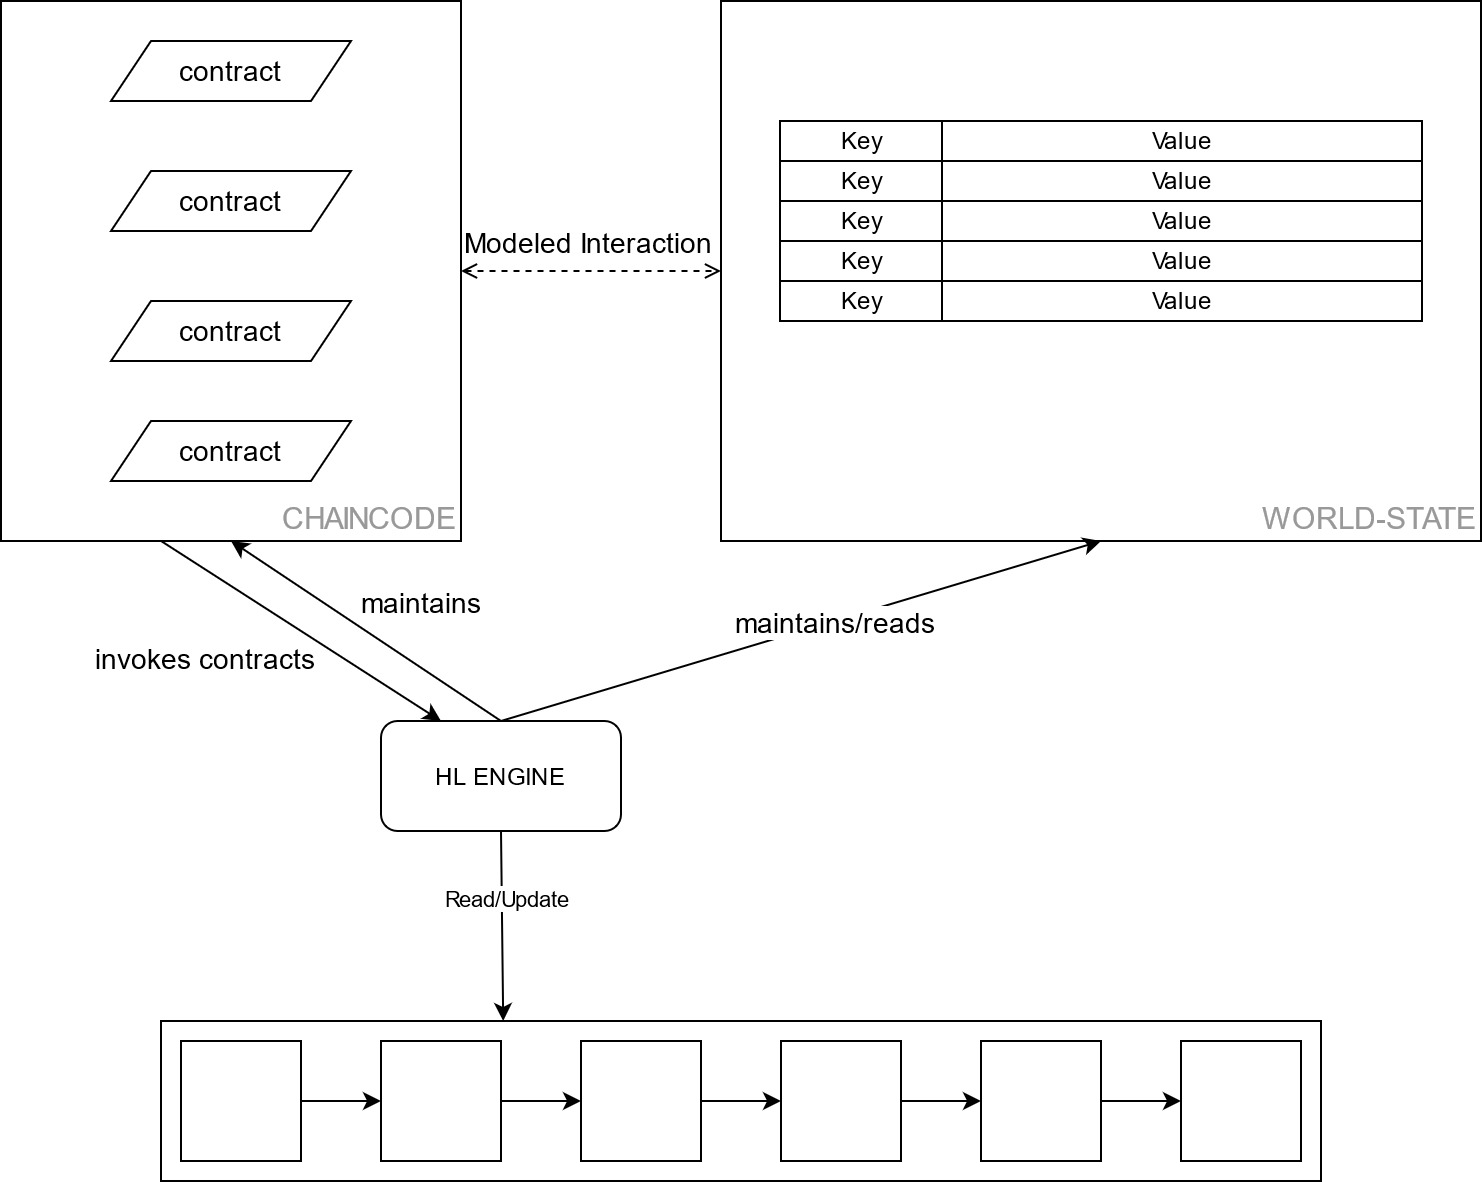
\includegraphics[height=0.7\textwidth]{gfx/hl-abstraction}
	\caption{Sketch of \emph{Hyperledger's} abstraction mechanism.}
	\label{fig:impr:hl:basics:abstraction}
\end{figure}

\textbf{Abstraction: \emph{World State \& Chaincode}} \\[0.2em]
As depicted in figure \ref{fig:impr:hl:basics:abstraction} by an 'engine' component (although this is a big simplification), Hyperledger has functions in place to display the underlying Blockchain's contents in a more abstract way, so that the user or developer doesn't need to bother with physical addresses, but may instead find them in a more human-readable format. \newline
The \emph{World State} Container is a synchronous representation of all data present in Hyperledger's underlying Blockchain, meaning that the data points present are always a representation their most recent update. Additionally, the World State is arranged like a dictionary, so that every structure inside is reachable by a key, defined by the user itself. This way, the programmer doesn't have to worry about physical addresses of the data. \newline
In the \emph{Chaincode} containers one can find the Smart Contract objects one would also find in other Blockchain application. However, these contracts are not stateful and therefore do not contain any data besides the location of the World State, where the data may be contained. In comparison, an \emph{Ethereum}-based contract may have private data and would therefore be stateful. Additionally, Chaincodes are also invocable via name, specifically by a combination of the parent contract name and the function that is to be executed.

\subsection{Component Overview}
\label{sec:impr:hl:requirements}

\begin{figure}[h]
	\centering
	\captionsetup{justification=centering,margin=2cm}
	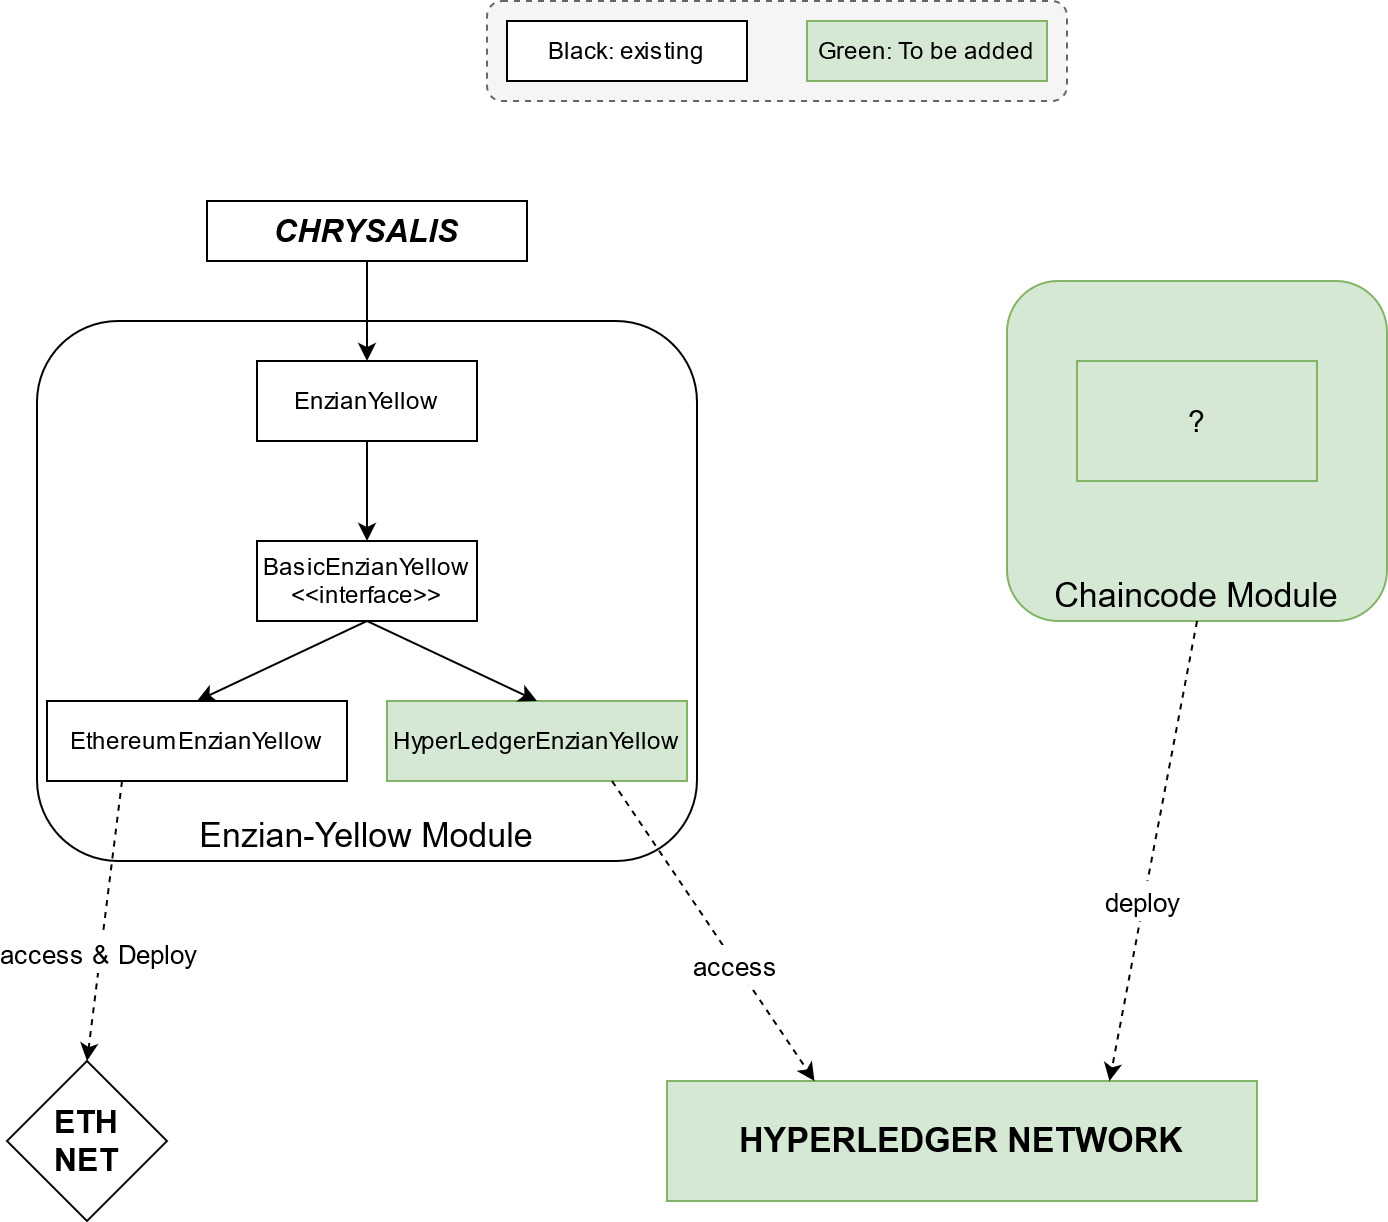
\includegraphics[width=\textwidth]{gfx/hl-structure}
	\caption{Planned and implemented module structure after adding the \emph{Hyperledger} protocol}
	\label{fig:impr:hl:structure}
\end{figure}

Three components will be needed to build a running Hyperledger-based application for the Chrysalis project. \newline
First of all, a Hyperledger Network must be established in the first place, so all necessary structures can be deployed there. Secondly, being the most complex component of the three, the Chaincode must be defined along with the data structures it uses. This module may be written and deployed in generic JavaScript thanks to Hyperledger's flexibility regarding the deployed language (e.g., this module could also be written in \emph{Go}). As per Hyperledger's requirements, the module must be contained in a separate package that can locally install dependencies and can be packed into a compressed file. Once this package is deployed, an API is needed in \emph{Enzian-Yellow} to access the Network and use the deployed components. This step is fairly straightforward, since Hyperledger Fabric provides this API and the structure of the \emph{HyperledgerEnzianYellow} can mostly be mirrored from that of \emph{EthereumEnzianYellow}.

\subsection{Test-Network}
\label{sec:impr:hl:network}

To keep development effort low, the Hyperledger Network where the contracts and data may be deployed was not built from scratch, but instead the "test-network" from Hyperledger's \emph{fabric-samples} repository was used. This network came with the features stated below.

\textbf{Network Deployment:} Instead of having to configure every network node, having to start it manually and registering it to the network, the test-network spares the developer from this work by making a running network with isolated components available as a composition of \emph{Docker}-Images. Additionally, with the help of pre-written scripts, the user may easily instantiate said composition.

\textbf{Reset functionality:} With a pre-written script, the developer may also simply wipe the entire network and bring it down. This makes development especially easy, since no trace (potentially even illegal states) of previous work will be left on the Blockchain.

\emph{Multi-Organization Scenario:} If instantiated with the right parameters, the network would come up with two organizations created, both containing one network peer each and reporting to a certificate authority. This configuration is useful, since the developer can make sure their application would run in a realistic scenario where their application and contracts must be validated by all network-registered organizations. The test-network also offers a lot of helpful scripts to make interactions with it a bit less cumbersome, e.g., so that Chaincodes may be deployed with less steps.

\subsection{Representation of Processes}
\label{sec:impr:hl:datastructure}

It makes sense to split the data model deployed onto the ledger into two parts: The first defines how a JavaScript object may be represented inside the \emph{World State} as well as in memory and how these two versions are to be synchronized. The second part, building on those definitions, defines how a process as well as it's tasks shall be modeled as such objects, how they interact and how they may be operated upon. The resulting components are visible in figure \ref{fig:impr:hl:data} and described below.

\textbf{Objects on the World State} \\[0.2em]
As the World State acts like a dictionary, any data placed on it is modeled as an extension of the class \emph{State}. This State object defines its own key with which it is found on said dictionary-like structure, as well as a static method to serialize and deserialize it to/from a JSON representation, as it has to be stored in a more permanent form. \newline
In addition to this data class, a 'manager' object is needed, in our case of the type \emph{StateList}, to store the location of the World State itself, to write or update deserialized State objects onto it, and to cast the 'rehydrated' objects back onto the correct class.

\begin{figure}[h]
	\centering
	\captionsetup{justification=centering,margin=2cm}
	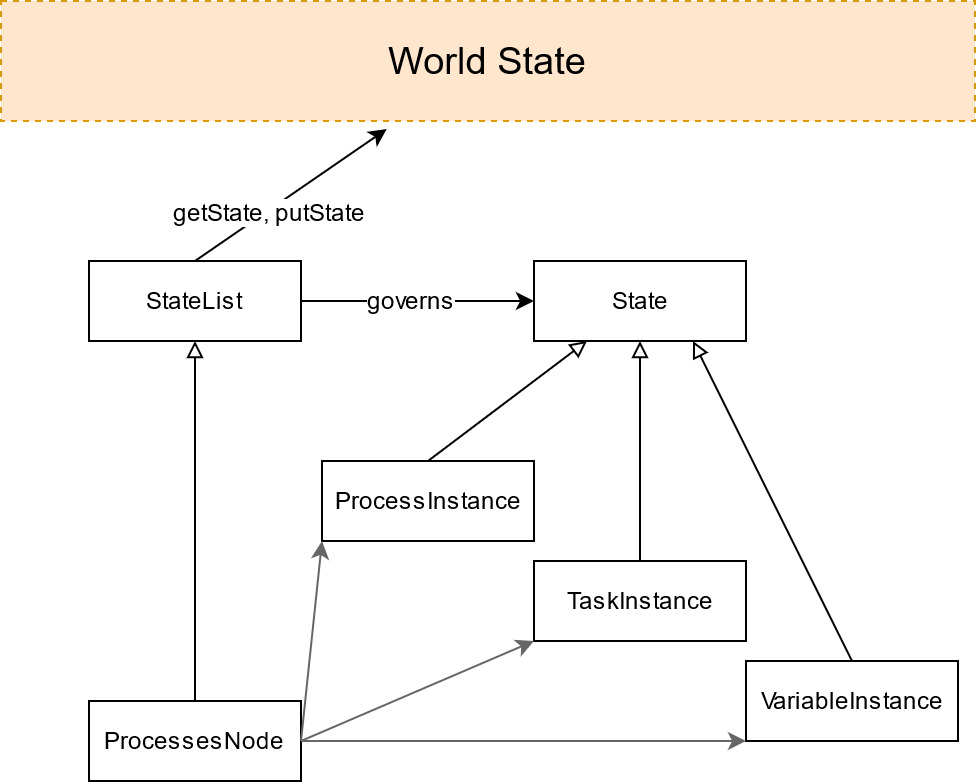
\includegraphics[width=0.8\textwidth]{gfx/hl-data}
	\caption{Data Structure deployed on the World State (State) as well as the objects that actively read and write on it (StateList)}
	\label{fig:impr:hl:data}
\end{figure}

\textbf{Process Representation} \\[0.2em]
With the definitions of \emph{State} and \emph{StateList} given, we can now implement the process structure as a simple extension of those, mostly not having to worry about the internals of the World State. 
\begin{itemize}
    \item \textbf{ProcessInstance}, being an extension of State, is the structure that binds an active process together: It stores the keys that point toward it's subordinated Tasks and Variables, and also contains the event log, which is an ordered list of task IDs, appearing in the order the tasks were executed (a newly created ProcessInstance would therefore contain an empty log). As the ProcessInstance is the 'root' object of the data structure, it's Key is simply defined as a positive integer.
    \item \textbf{TaskInstance}, representing the Task State, contains - besides it's key and ID - all necessary data that makes up tasks in BPMN: A name, a list of competing tasks and completed task IDs required for execution, and so on. Additionally, to model BPM gateways it contains a \emph{precedingMergingGateway} attribute as well as a \emph{decision} structure, similar to the structures defined in the Ethereum application. The key is defined as follows: \emph{[key of parent process]:task:[task ID]}
    \item \textbf{VariableInstance}, lastly, is a simple wrapper for a value of a given type, with a log of previous values as an addition. Currently, only variables of type integer and string are supported. The key is defined as follows: \emph{[key of parent process]:var:[variable ID]} - also showing why the middle section differentiating between tasks and variables is needed: Variable and task IDs may clash and must therefore be expanded by some prefix.
\end{itemize}
The \textbf{ProcessesNode} class, extending StateList, acts as a gateway to the previously defined objects, offering the usual \emph{get, set} and \emph{update} methods. Also, since it makes sense to immediately write every action on the data structure onto the World State after executing it to prevent bugs, ProcessesNode also offers many BPM-based functions like \emph{executeTask}, therefore encapsulating a lot of Process logic as well. Objects of this class are meant to make it possible to interact with the process model entirely without knowing the underlying model, only using provided keys. \newline
How this ProcessesNode finds its way into a Chaincode, however, will be explained in the next chapter.

\subsection{Process Deployment and Execution}
\label{sec:impr:hl:chaincode}

A Smart Contract (Chaincode) in Hyperledger Fabric, as well as the data structure, can be written in multiple supported programming languages, including JavaScript, which was used here. Implementing it is as simple as creating a class that extends the \emph{Contract} class from the Fabric API, as seen in figure \ref{fig:impr:hl:contract}.

\begin{figure}[h]
	\centering
	\captionsetup{justification=centering,margin=2cm}
	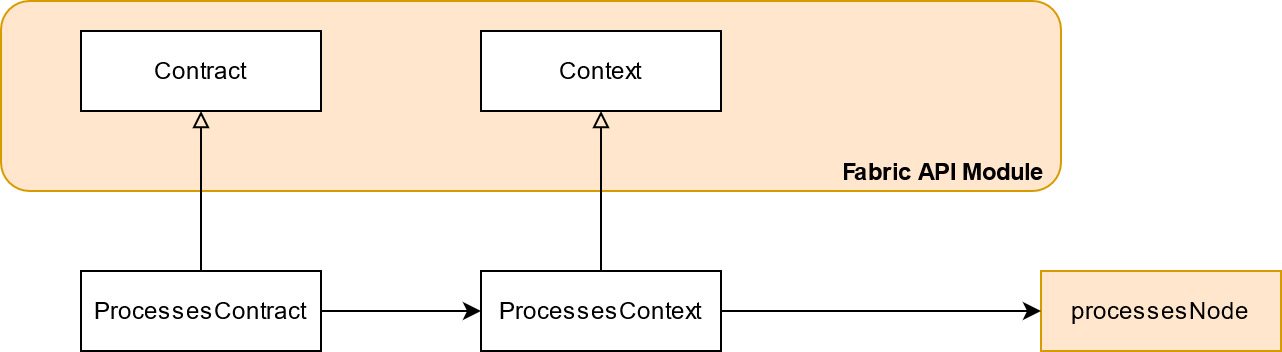
\includegraphics[width=\textwidth]{gfx/hl-contract}
	\caption{Structure of a Chaincode (Contract) together with it's gateway object that points to the World State (Context)}
	\label{fig:impr:hl:contract}
\end{figure}

\textbf{Contracts} \\[0.2em]
Defining what would be an invocable contract from the outside is as simple as giving the extending \emph{Contract} class a method: Users will be able to invoke this function simply by its name coupled with the class's name, e.g., "ProcessesContract" and "createProcess", together with it's arguments. However, a few special rules apply here: Firstly, while parameters and return values can be generic JavaScript objects that do not have to be serialized, all non-primitive types must be transferred via \emph{Buffer} to account for the networking between the caller and the callee. Secondly, the contract methods will always be provided a \emph{Context} object (see next passage for details) as first positional argument. This context will be handed to the method by the Hyperledger API, not the caller, therefore only the second argument and all those after may be used for argument passing.

\textbf{Context} \\[0.2em]
The Context, as described before, is another object provided by Hyperledger's API and handed to every smart contract during execution. Foremost, it contains the network-\emph{stub}, which is the gateway to the World State. We can now extend this Context into \emph{ProcessesContext}, that always contains a newly instantiated ProcessesNode object, therefore also giving access to all the data structures and logic as we defined them in section \ref{sec:impr:hl:datastructure}. During instantiating, the ProcessesNode is also handed a reference to the stub, so that it may have an access point to the World State. To make clear to Hyperledger's API that our Chaincode is supposed to use this version of Context, we override the Chaincode's method \emph{createContext} to return our version instead of the default one. 

With these two components, it is now clear how a contract invocation results in manipulations or queries on the processes: When a method of ProcessesContract is invoked, it is handed the ProcessesContext and uses it to access ProcessesNode to then execute all process-related logic there. The whole interaction is currently purely based on passing and returning keys and primitive construction parameters, however it would also be possible for the caller to receive objects from the data structure as copies of their current state - still, it should generally be disallowed to write self-made objects to the network, as this might cause trust issues.

\subsection{Integration into Chrysalis}
\label{sec:impr:hl:integration}

From the side of HyperledgerEnzianYellow, interaction is fairly simple. Due to the underlying interaction model in the Hyperledger network being similar to the model deployed to the \emph{Ethereum} network, the general structure of HyperledgerEnzianYellow is basically the same as that of EthereumEnzianYellow. \newline
When HyperledgerEnzianYellow is instantiated, the HyperledgerAccessor is also constructed, building up a working connection to the Hyperledger network during construction (or throwing, if the connection fails). Currently, provided arguments aren't used, but instead read from a static definition, as an integration error (see section \ref{sec:issues:integration}) made using it properly impossible. \newline
Once the connection is built, the accessor can then freely pull a Chaincode by simply specifying the correct name, being returned an interface object. This interface can then be used to invoke the contracts by name and handing over parameters, as if the method were local. Using the previously defined Chaincode, HyperledgerEnzianYellow can offer the same functionality for BPM as EthereumEnzianYellow with the same parameters, the only difference being that the process addresses are in fact structured keys instead of proper addresses.

\subsection{Result}
\label{sec:impr:hl:result}

All in all, the task of implementing a Hyperledger-based process execution engine as a prototype can be considered successful and fruitful. The Hyperledger Smart Contracts are able to mirror the Ethereum Contracts, can be deployed on a running system successfully and can be connected to - especially by HyperledgerEnzianYellow. From a BPM perspective, the Hyperledger application fulfills all required functions and even partly surpasses Ethereum in a few features:
\begin{itemize}
    \item \textbf{Execution Speed:} As Hyperledger doesn't rely on mining to sign and validate new additions to the Blockchain, the deployed contracts can be invoked with fairly low delay - about two seconds per invocation. A direct comparability with Ethereum is not given, though: A mining-based protocol can technically be sped up massively by adding more miners and reducing the hashing difficulty of the mining puzzles. Still, Hyperledger's test-network is rather feature-rich and probably contains a lot of overhead that might not be needed in our case, and might also be a lot quicker if optimized.
    \item \textbf{Reliability:} Compared to a mining blocks, adding them after a consensus is not based on random numbers. Therefore, the time between a contract invocation and the completion of the underlying transaction is extremely constant. In Ethereum's case, we saw huge discrepancies between the times individual transmissions took.
    \item \textbf{Readability:} As a small bonus, all addresses Hyperledger uses - even internally - are developer-defined and therefore have a human-readable structure, like those of the process data structure defined in section \ref{sec:impr:hl:datastructure}, and therefore make development and back end work a lot easier and more transparent even without usage of a persistence layer.
    \item \textbf{Efficiency:} Without mining, we perceived a significant reduction in processing load on the Hyperledger application compared to the Ethereum one. For example, where the Hyperledger application occupied a few threads with barely any load on the processor, the Ethereum miner alone (before process Chrysalis even ran), needed to put multiple processor cores on full load only to facilitate a transaction delay low enough to comfortably work with. This issue might not arise on more powerful server architectures, though.
\end{itemize}